\documentclass{article}
\usepackage[T1]{fontenc} %Better support for european accented chars
\usepackage[utf8]{inputenc} %Enables danish chars and other good stuff
\usepackage{lmodern} 
\usepackage{amssymb}
\usepackage{csquotes} % qoute in danish
\usepackage[danish]{babel}
\usepackage{pstricks-add}
\usepackage{lastpage} %Package for getting the number of the last page.
\usepackage{graphicx} %Allows insertion of graphics
\usepackage{amsmath} %Gives better math support.
\usepackage{amsfonts} %Gives additional fonts.
\usepackage{amssymb} %Adds additional symbols.

%Pakker der bruges for at lave klikbare links i pdf filer
\usepackage{varioref} %Gives the \vref{lbl} command that make nice references that includes page numbers.
\usepackage[pdftex, colorlinks=false, pdfauthor={\authorText}, pdftitle={\titleText}]{hyperref} %Makes references clickables in the pdf file. colorlinks can be set to true for colored links.
\usepackage{memhfixc} %Solves problems with hyperref in Memoir, to be loaded after hyperref.

\usepackage{url}
\usepackage{pdfpages}
\usepackage{listings}
\usepackage{color}
\usepackage{url} % Nice url look
\usepackage[backend=bibtex,style=alphabetic]{biblatex} %Bibliography package.
%\usepackage{anysize}
%\marginsize{3cm}{3cm}{1.5cm}{4cm} % venstre, højre, top, bund.
\lstset{literate=%
{æ}{{\ae}}1
{å}{{\aa}}1
{ø}{{\o}}1
{Æ}{{\AE}}1
{Å}{{\AA}}1
{Ø}{{\O}}1
}

\definecolor{mygreen}{rgb}{0,0.6,0}
\definecolor{mygray}{rgb}{0.5,0.5,0.5}
\definecolor{mymauve}{rgb}{0.5,0,0.3}
\definecolor{myblue}{rgb}{0,0.4,0.9}
\pagestyle{plain}

\bibliography{19_del3} %Choose the bibliography to load, file to be called name.bib.

\begin{document}
\section*{Projektopgave efterår 2013 - jan 2014}
\section*{02312-14 Indledende programmering og 02313 Udviklingsmetoder til IT-Systemer}
Projektnavn: \textcolor{red}{del3}
Gruppe nr: \textcolor{red}{19}
Afleveringsfrist: \textcolor{red}{mandag den 02/12 2013 Kl. 5:00}
\\\\
Denne rapport er afleveret via Campusnet (der skrives ikke under)
\\\\
Denne rapport indeholder \textcolor{red}{77} sider incl. denne side
\\\\
Studie nr, Efternavn, Fornavne
\\\\
\textcolor{red}{s110795, Mortensen, Thomas Martin}
\\
Kontakt person (Projektleder)
\\\\
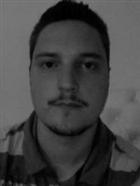
\includegraphics[scale=0.5]{ThomasM.jpg}
\\\\
\textcolor{red}{s113577, Johansen, Chris Dons}
\\\\
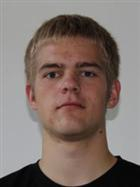
\includegraphics[scale=0.5]{ChrisJ.jpg}
\\\\
\textcolor{red}{s123897, Ahlgreen, Thomas Kamper}
\\\\
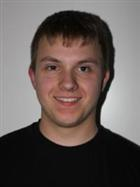
\includegraphics[scale=0.5]{ThomasA.jpg}
\newpage
\section*{Timeregnskab}
\begin{tabular}{|c|c|c|c|c|c|c|r|} \hline
 Dato & Deltager & Design & Implementering & Test & Dok. & Andet & I alt \\ \hline
&&&&&&& \\ \hline
 15/11-13 & Thomas Mortensen & 2& & & & & 2\\ \hline
 15/11-13 & Chris Johansen & 2& & & & &2 \\ \hline
 15/11-13 & Thomas Ahlgreen & 2& & & & & 2\\ \hline
 &&&&&&& \\ \hline
 22/11-13 & Thomas Mortensen & & 2,5& & & &2,5 \\ \hline
 22/11-13 & Chris Johansen & &2,5 & & & &2,5 \\ \hline
 22/11-13 & Thomas Ahlgren & & 2,5& & & &2,5 \\ \hline
 &&&&&&& \\ \hline
 29/11-13 & Thomas Mortensen & &2,5 & & & &2,5 \\ \hline
 29/11-13 & Chris Johansen & &2,5 & & & & 2,5 \\ \hline
 29/11-13 & Thomas Ahlgren & &2,5 & & & & 2,5 \\ \hline
 &&&&&&& \\ \hline
 2/12-13 & Thomas Mortensen & & &1 &6 & &7 \\ \hline
 2/12-13 & Chris Johansen & & &1 &6 & &7 \\ \hline
 2/12-13 & Thomas Ahlgren & & &1 &6 & &7 \\ \hline
 &&&&&&& \\ \hline
 diverse & Thomas Mortensen & & & &4 & & \\ \hline
 diverse & Chris Johansen & & & & &2 & \\ \hline
 diverse & Thomas Ahlgren & & & & & & \\ \hline
 &&&&&&& 48\\ \hline
\end{tabular}
\newpage
\tableofcontents
\newpage
\section{Indledning}
Spilfirmaet IOOuterActive har givet os endnu en opgave.

Kundens vision er en udvidelse af vores allerede udviklede programmer fra \cite{19del1} og \cite{19del2}

Denne gang ønsker kunden at lave flere forskellige typer felter. Disse felter skal implementeres på en "rigtig" spilleplade, hvor man kan gå i ring. Samtidig ønskes der mulighed for 2-6 spillere. Spillerens konto skal sættes med et fast beløb fra start, og spillet skal slutte, når en spiller er gået bankerot.


Projektet forventes at have elementer fra både \textbf{FURPS+} og \textbf{GRASP}. Herudover er der lavet specifikke krav til hvilke artefakter, der skal ingå i krav, analyse, kode, test, og designdokumentation.
\\

OBS: alle gruppemedlemmer er lige ansvarlige for alle dele af vores dokumentation
\section{Kravspecificering og Use cases}
I dette afsnit vil vi beskrive vores kravspecificering og vores Use cases, som vi har udarbejdet til denne rapport.
\subsection{Kravspecificering}
I dette afsnit har vi taget udgangspunkt i kundens vision. Vi har læst den igennen, og stillet spørgsmålstegn, ved de ting, der kunne være tvivl om. Kunden er dog blevet til kravspecificering i forløbet, og derfor var der få tvivlsspørgsmål.
\begin{enumerate}
\item Hvad skal der ske, hvis en spiller ikke kan betale det han skal?
\item Skal man betale, hvis man lander på et felt, der er ejet af en bankerot spiller?
\item Skal man have mulighed for at købe eet felt, der tidliger var ejet af en spiller, der nu er gået bankerot?
\end{enumerate}
Vores kontakt i firmaet, som er vores projektleder, har besvaret disse punkter på følgende måde
\begin{enumerate}
\item Spilleren der ikke kan betale, må betale det han har, og går herefter bankerot.
\item Feltet er ikke længere ejet af nogen, og derfor skal der heller ikke betales.
\item Da feltet ikke længere ejes, skal man kunne købe det.
\end{enumerate}
\newpage
\subsection{Fully Dressed Use Case}
Vi har i dette afsnit beskrevet vores use case med en fully dressed use case for Fleet.
\subsubsection*{Use Case}
Fleet
\subsubsection*{Scope}
Spil
\subsubsection*{Level}
Bruger Konsekvens
\subsubsection*{Primary actor}
Spiller
\subsubsection*{Stakeholders and Interests}
Spiller: Vil købe felt
\subsubsection*{Preconditions}
Eclipse er installeret på maskinen.
\\
Programmet er kørende.
\subsubsection*{Main Success Scenarie:}
\begin{enumerate}
\item[1] Spiller starter spillet
\item[2] Spiller indtaster Navn
\item[3] Spiller Ruller med terningerne
\item[4] Spiller lander på Fleet
\item[5] Spiller køber Fleet
\item[6] System checker pengebeholdning
\item[7] System trækker penge
\item[8] System giver turen til næste spiller
\end{enumerate}
\subsubsection*{Extensions Alternative scenarier:}
*a - til hvert et tidspunkt
\begin{enumerate}
\item Spiller lukker spillet ved at taste "q"
\end{enumerate}
5a. Spiller skal betale penge
\begin{enumerate}
\item  Spiller betaler regning
\end{enumerate}
5b.
\begin{enumerate}
\item  Spiller kan ikke betale
\item  System giver turen videre
\end{enumerate}
\subsubsection*{Specielle Krav:}
\begin{itemize}
\item Skal kunne køre på en Windows maskine med Java EE på DTU's computere
\item Skal kunne spilles af en almindelig bruger
\end{itemize}
\subsection{Refuge Brief}
Når en spiller lander på refuge, skal spilleren (afhængigt af om de lander på Walled City eller Monastery) modtage hhv. 5000 eller 500.  
\subsection{Fleet Test Brief}
En udvikler sætter testen igang. Når testen er igang tester den hvor meget man skal betale ud fra flere scenarier.
\subsection{Refuge Test Brief}
Denne test, tester om man faktisk får penge når man lander på feltet. Den tester også om hvorvidt der returneres forventede beløb.
\newpage
\section{FURPS+}
I \textbf{UP} bruger man \textbf{FURPS+}, der er udviklet af Hewlett-Packard til at kategoriserer kravene til ens system. "\textbf{+}" i \textbf{FURPS+} kom i følge \cite{WikiFURPS} til senere, efter HP ønskede at dække flere kategorier med denne model. Vi har beskrevet kort, hvad der generelt hører under de forskellige punkter i \textbf{FURPS+}, og efterfølgende listet de funde krav i den aktuelle opgave op.
\subsection{Functional}
Hvilke funktioner skal systemt have. Hvad skal det kunne. Sikkerhed.


Vi har taget udgangspunkt i kundens \cite{CDIO3} opgave. Ud fra deres vision, bilag og andre punkter i rapporten har vi fundet frem til følgende punkter:
\begin{itemize}
\item En udbyggelse af forrige system med forskellige felttyper.
\item En spilleplade, hvor spillerne skal kunne lande på et felt og fortsætte på næste slag. Samtidig skal man kunne gå i ring på brættet.
\item Man skal kunne vælge mellem 2-6 spillere.
\item Et \textit{Territory} skal kunne købes af en spiller, når han lander på feltet. Feltet skalhave en fast leje. Jo højere feltnummer jo højere pris og leje.
\item Et \textit{Refuge} skal give en bonus på enten 5000 eller 500 afhængigt af feltnummeret, når en spiller lander på denne type felt.
\item Når man lander på et \textit{Labor Camp} felt, skal man betale 100 gange værdien af et nyt terningeslag. Dette beløb skal i øvrigt ganges med antallet af \textit{Labor Camps} med den samme ejer.
\item Der er to felter af typen \textit{Tax}. Det ene felt betaler man et fast beløb af Kr. 2000,-, når man lander på feltet. Det andet skal man selv vælge om man vil betale et fast beløb af Kr. 4000,- eller om man vil betale 10\% af hele sin formue. (Hvilket betyder, både af hvad der står på kontoen og af felter man ejer).
\item Lander man på et felt af typen \textit{Fleet}, bestemmes beløbets størrelse ud fra hvor mange \textit{Fleet} felter, der har samme ejer.
\end{itemize}
Sikkerhed er et punkt, vi ikke kan finde noget om, så vi må gå ud fra firmaet selv sørger for dette.
\subsection{Usability}
Menneskelige faktorer, skal man bruge hjælp. Dokumentation af systemet i brug.


Vi går ud fra, at kravene til \textbf{Usability} er de samme som i foregående opgaver. Det er kun dokumentation, der er nævnt i denne opgave. Kravene fra sidst, var at det skulle kunne bruges af en normal person med en 9. klasses eksamen. Der må ikke være brug for hjælp. Dog må man godt forklare hvad spillet går ud på.

Til dokumentation forventes der \textbf{Designsekvensdiagrammer}, der viser den dynamiske tilgang til programmet.
\subsection{Reliability}
Hyppigheden af fejl, kan det nemt gendannes og forudsigelighed.


For at formindske hyppigheden af fejl, har vi løbende brugt User Test, for at fange semantiske fejl. Herudover har IOOuterActive stillet en skabelon til\textbf{Junit} tests, der gerne skulle fange fejl i vores \texttt{Field} klasser. Derudover er der ikke nogle målbare krav til \textbf{Reliability}.
\subsection{Performance}
Responstider, informationer i systemts gennemløb, præcision, tilgængelighed af systemet og hvor mange ressourcer må det bruge.


Vi går ud fra tilgængeligheden er det samme som i de andre opgaver. Her var kravet, at programmet skulle kunne køre på maskinerne i \textbf{DTU}'s databarer.
\subsection{Supportability}
Ændringer, vedligeholdelse, internationalisering og konfigurationsmuligheder.


Her anbefales det at vi så vidt muligt overholder \textbf{GRASP} patterns og samtidig benytter os af \textbf{FURPS+}. Dette skulle gerne gøre programmet nemmer i forhold til alle punkter i \textbf{Supportability}.
\subsubsection*{Her kommer de underfaktorer, som +'et repræsenterer}
\subsection{Implementation}
Ressource begrænsninger, sprog, værktøjer og hardware


Her er igen ikke nogle direkte krav. Vi går ud fra, at afleveringsproceduren er den samme som i foregående opgaver. Det vil betyde at projektet skal afleveres som et \textbf{Eclipse} projekt
\subsection{Interface}
Begrænsninger fremkommet af at skulle interagere med grænseflader fra eksterne systemer.


Den eneste begrænsning vi har er på den udleverede \textbf{GUI}, da vi ikke selv har udviklet denne. Vi kan derfor benytte os af allerede implementerede funktioner i denne.
\subsection{Operations}
Sporing og kontrollering af ændringer i softwaren.


Det er ikke noget vi skal tage stilling til i dette projekt.
\subsection{Packaging}
Hvordan skal programmet leveres (Fysisk eller fil)? Hvor mange installationer er der.


Igen går vi ud fra tidligere opgaver, hvor vi skulle aflevere programmet elektronisk, som et pakket \textbf{Eclipse} projekt også indeholdende vores rapport. Vi skal ikke installere det for kunden.
\subsection{Legal}
Licensering med videre.


Det er ikke noget vi er gjort opmærksom på af IOOuterActive. Det eneste vi kan nævne i forhold til retsmæssige stridigheder er, at vi skal tillade brugen af vores materiale, hvis dette ønskes benyttet til f.eks. undervisningssituationer.
\section{Domænemodel}
Vi har i denne omgang valgt at modificere på vores \textbf{Domæne Model} fra \cite{19del2}, da denne allerede fungerede ret godt. Vi har dog måttet tilføje de nye domæner, som IOOuterActive har leveret i form af deres vision.


Vi kan se at det eneste ekstra domæne vi har tilføjet er \textit{Field}. Vi kunne have valgt at lave domæne klasser til vores forskellige felttyper også, men på den måde ville man hurtigt miste overblikket. Vi vurderede at det vigtigste var at vores kunde også ville kunne forstå modellen. Herudover har vi flyttet lidt rund på relationerne mellem domænerne. Før var det \textit{Game}, der kendte til \textit{DieCup}, men i denne omgang valgte vi at sige, det var mere logisk at man brugte raflebægeret på spillebrættet, hvilket nok er mere tro mod virkeligheden. Dette ses i figur \vref{fig:domain}

\begin{figure}[!ht]
    \centering
    \includegraphics[width=1\textwidth]{Domainmodel.pdf}
    \caption[<Text for the list of figures>]{Domæne Model}
    \label{fig:domain}
\end{figure}
\newpage
\section{BCE model}
I dette, har vi opfyldt kravet omkring en BCE model til at dokumentere og skabe oveblik over vores kendskab i koden.


Vi har igen brugt \texttt{Game} som vores \textit{Controller}, der uddeler ansvaret til de andre klasser. Ud over det er det de samme \textit{Entities} og \textit{Boundaries}, som i \cite{19del2}.

I forhold til en optimal \textbf{BCE model}, har måttet ændre lidt i dens kendskaber. Efter at have sammenlignet koden med vores udgangspunkt, har vi måttet lave kendskab begge veje mellem \texttt{Gameboard} og \texttt{Field}. Samtidig fik vi et krav i opgaven, at \texttt{Field} skulle kunne kalde objekter af \texttt{Player}. Derfor har vi også måttet lave et kendskab der.

Kendskabet til \texttt{DieCup} har vi flyttet over i \texttt{GameBoard}, for at få det til at passe med vores nye \textbf{Domæne Model}, og for at sørge for \texttt{Game} ikke blev bloated af ansvarsopgaver.

Overblikket over dette kan ses i figur \vref{fig:bcemodel}

\begin{figure}[ht]
\centering
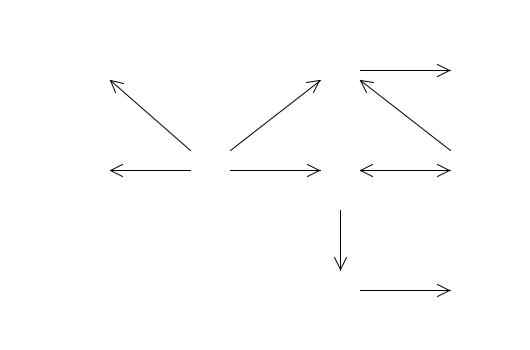
\includegraphics[width=1\textwidth]{BCEModel.pdf}
\caption[<Text for the list of figures>]{BCE Model}
\label{fig:bcemodel}
\end{figure}
\newpage
\section{Systemsekvens Diagram}
Et \textbf{SSD} er til for at få en indsigt i, hvordan et program ser ud. I dette diagram kan det ses, hvordan systemet kom til at se ud baseret på krav fra kunden.

I diagrammet ses det, at så snart et spil er startet, bliver nogen forskellige ting oprettet (ligesom i et bræt spil i virkeligheden). Der uddeles nogen penge til hver spiller og mængden af spillere. 
Spillet kørers så, som det ses i \vref{fig:ssd}. landOnField er tilføjet for at man kan se at det har en konsekvens at lande på et felt. Vi har for overblikket skyld ikke lavet returveje fra systemet på samtlige typer af felter, da det hurtigt kunne blive uoverskueligt for kunden. 

Alt hvad der står i loop'en sker om og om igen indtil spillet er forbi ved at alle på nær 1 spiller er gået falit. Når en spiller er tilbage erklæres han vinder og spillet kan lukkes.
\begin{figure}[!ht]
\centering
\includegraphics[width=0.6\textwidth]{SSD.pdf}
\caption[<Text for the list of figures>]{Systemsekvens Diagram}
\label{fig:ssd} 
\end{figure}
\newpage
\section{Kode}
Her vil vi forklare hvordan vi har grebet selve koden an.
\subsection{Struktur og pakker}
Ligesom i de to foregående projekter, er programmet skrevet med fokus på at overholde \textbf{BCE}-modellen. Kort fortalt betyder det for opdelingen i pakker, at alle klasser er inddelt i pakker efter deres type ift. \textbf{BCE}. For en mere uddybende beskrivelse henvises til det tilsvarende afsnit i \cite{19del1} og \cite{19del2} rapporterne.
\subsection{Genanvendelse af kode og opbygning}
På baggrund af hensigtsmæssigt og godt design i \cite{19del1} og \cite{19del2} projekterne, har det været muligt at genbruge store dele af koden. Således er klasserne \texttt{Die} og \texttt{DieCup} i praksis identiske med de tilsvarende klasser fra de tidligere projekter, ligesom den generelle opbygning af systemet også ligner meget.

På samme måde er det grundlæggende princip bag \texttt{TUI} og \texttt{Graphic} klasserne også identisk med 19del2 – klasserne har ikke behov for at bære data, og de forskellige metoder i klasserne interagerer ikke med hinanden gennem felter eller lign, og kan derfor med fordel være statiske. For en mere dybdegående forklaring henvises til kodeafsnittet i 19del2.

\subsection{Bemærkelsesværdige løsninger}
Systemet er på nuværende tidspunkt så omfattende, at det ikke giver mening at gennemgå alle overvejelser bag implementeringen af alle klasser. I stedet uddrages specielt bemærkelsesværdige dele af koden, og forklares herunder, for at give en bedre forståelse af systemets virkemåde, uden at gennemgå alt. Beskrivelserne er opdelt efter hvilke klasser de er implementeret i.
\subsubsection{TUI}
Noget af det første der sker, når dette spil startes, er at brugeren anmodes om at indtaste antallet af spillere. Antallet af spillere må ifølge opgavebeskrivelsen ikke være større end 6, og spillet giver ikke meget mening, hvis det er mindre end 2. Med andre ord skal der specifikt indtastes et tal mellem 2 og 6. Dette er en ny udfordring ift. de tidligere opgaver, hvor der blot blev gemt en hel streng. Foruden at teste, at det indtastede tal er i det krævede interval, ønskede vi også at lave systemet robust, og sikre at f.eks. bogstaver eller specialtegn indtastet på dette tidspunkt, ikke kunne få systemet til at gå ned. Dette ses i figur \vref{fig:kode1}.
\begin{figure}[!ht]
\centering
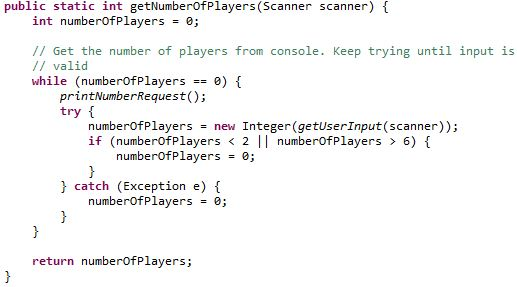
\includegraphics[width=0.8\textwidth]{kode1.jpg}
\caption[<Text for the list of figures>]{Antal spillere}
\label{fig:kode1} 
\end{figure}
Tjekket og sikringen mod karakterer som ikke er tal, sker i \texttt{TUI}, inden det sendes videre til controlleren. Antallet af spillere sættes indledningsvist til 0, og forespørgslen kører så i en løkke, som kun brydes når antallet af spillere bliver sat til noget der er forskelligt fra 0. Det input der hentes fra konsollen er som udgangspunkt en streng, og skal derfor konverteres før det kan bruges som en talværdi. Denne konvertering vil kaste en Exception, hvis der gives et input, der ikke umiddelbart giver mening som tal-værdi – f.eks. et bogstav. Det smarte er så, at denne Exception kan fanges, og kode kan udføres til at ”reparere” den fejl, som har forårsaget den. I vores tilfælde sætter vi bare værdien for antal af spillere tilbage til 0, fordi det betyder at løkken kører igen, så brugeren bliver spurgt efter et nyt input.
Ligeledes hvis der gives et input, som succesfuldt kan konverteres til en talværdi, tjekkes der om tallet er mellem 2 og 6 – hvis ikke det er det, sættes værdien tilbage til 0, og løkken kører igen. Så snart løkken brydes, returnerer metoden.

\subsubsection{GameBoard}
Ligesom ved et fysisk spil, indeholder dette system en spilleplade \texttt{GameBoard}, som er bygget op af felter af forskellig type. Disse felter er bygget i et system med arv, som beskrevet senere i dette afsnit, og dette giver en stor fordel for datastrukturen i \texttt{GameBoard}. Fordi alle de forskellige felttyper \texttt{Territory, LaborCamp, Fleet, Tax og Refuge} nedarver fra Field, kan der laves en enkelt liste (array) af felter, af typen \texttt{Field}, som kan indeholde alle de forskellige felter, selvom der er tale om forskellige typer objekter, med forskellige implementeringer af metoder mm. Koden ses i figur \vref{fig:kode2}.
\begin{figure}[!ht]
\centering
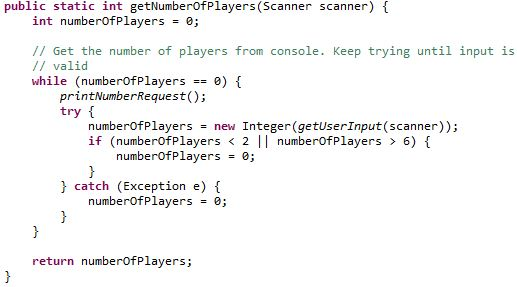
\includegraphics[width=0.8\textwidth]{kode1.jpg}
\caption[<Text for the list of figures>]{Antal spillere}
\label{fig:kode2} 
\end{figure}
\subsubsection{Field} 
Som nævnt tidligere, er felterne bygget op med at system af arv. Alle felterne nedarver fra \texttt{Field}, som indeholder de ting der er fælles for alle felter. I realiteten er det ikke ret meget der er det samme for alle felter – der er forskellige muligheder ift. køb, der er forskellige konsekvenser (få penge, miste penge), og selv de felter der har den samme konsekvens – at man skal betale til andre – har forskellige måde at beregne beløbet på.

Alle felter har dog et navn, og alle felter har mulighed for at man kan lande på dem. Derfor indeholder \texttt{Field} et felt til navn, og en abstrakt metode – \texttt{landOnField} – der betyder at alle klasser som arver fra \texttt{Field}, skal ”love” at de implementerer \texttt{landOnField}. De forskellige underklasser kan så have forskellige implementeringer af \texttt{landOnField}, så længe typen af parametre og returværdi er de samme.


To typer felter – \texttt{Tax} og \texttt{Refuge} – nedarver direkte fra \texttt{Field}, men de resterende 3 felttyper nedarver i stedet fra \texttt{Ownable}, som så igen nedarver fra \texttt{Field}. Dette skyldes, at disse 3 felter – \texttt{Territory, LaborCamp} og \texttt{Fleet} – kan købes. Dette er en funktionalitet, som grundlæggende vil virke ens for alle tre typer felter – der skal være et pegepind til en ejer, der skal være en måde at købe feltet osv.
Desuden vil den grundlæggende procedure, når der landes på feltet, også være ens – der skal tjekkes om der er nogen der ejer feltet, og hvis der er, skal der betales leje til ejeren. Hvordan lejen udregnes, er forskellige for de forskellige typer at felter, men den overordnede procedure er ens. Derfor er \texttt{landOnField}-metoden, der som bekendt skal implementeres, når klasserne arver fra \texttt{Field}, implementeret i \texttt{Ownable}. Metoden i \texttt{Ownable} kalder så \texttt{getRent-metoden}, der har forskellig implementering i hver af underklasserne.
\subsubsection{Fleet}
Af de underklasser, hvor der skal udregnes leje, er \texttt{Fleet} en af de mere interessante. Lejen for \texttt{Fleet} afhænger nemlig af hvor mange andre \texttt{Fleet}-felter ejeren af det felt der landes på, har. Det betyder, at det \texttt{Fleet}-felt der er landet på, er nødt til at kende ejeren af de øvrige \texttt{Fleet}-felter, for at kunne udregne lejen.
I praksis implementeres det ved, at et \texttt{Fleet} felt-objekt tager den spilleplade \texttt{GameBoard} det oprettes i, med som parameter, når det oprettes. Således har \texttt{Fleet}-feltet mulighed for at gå ud og se på andre felter på den samme spilleplade.

Dernæst er problematikken blot, at de objekter på spillepladen, som dette objekt nu har adgang til, er af typen \texttt{Field}. Overklassen \texttt{Field} indeholder ikke en ejer, så før ejeren af feltet kan findes, må det konverteres til \texttt{Ownable}. Herefter er det blot en simpel løkke, som tjekker ejeren på hvert \texttt{Fleet}-felt, og summerer op. Når antallet af \texttt{Fleet}s er fundet, kan lejen simpelt findes med en switch-sætning.
\subsubsection{LaborCamp}
På samme måde som \texttt{Fleet}, bruges antallet af ejede felter af samme type også til beregningen af lejen ved \texttt{LaborCamp}. Fremgangsmåden til at finde antallet af ejede felter, er helt den samme som ved \texttt{Fleet}.
Foruden antallet af ejede \texttt{LaborCamps}, indgår også et terningslag i beregningen af lejen – det betyder at \texttt{LaborCamp} er nødt til at have kendskab til \texttt{DieCup}, for at kunne få værdien af et terningslag. Imidlertid befinder\texttt{DieCup} sig på spillepladen \texttt{GameBoard}, så i kraft af at \texttt{LaborCamp} allerede har \texttt{GameBoard} med som argument, for at kunne kigge på andre felter, har den også let adgang til \texttt{DieCup}.
\subsubsection{Ownable}
Som nævnt tidligere i afsnittet, er der 3 felttyper som kan købes. Nå en spiller køber et felt, skal der trækkes nogle penge fra spillerens konto, og \texttt{owner}-pegepinden i feltet skal sættes til at pege på spillerens objekt. Før dette sker, skal der imidlertid have været præsenteret et valg for spilleren, om hvorvidt denne ønsker at købe feltet eller ej, og lige netop dette viser sig at være den mest krævende del at implementere af denne funktionalitet.


Ideen med hele opbygningen af systemet efter \textbf{BCE}-modellen er nemlig, at elementer fra entitets-laget aldrig har direkte adgang til elementer fra brugergrænseflade-laget. Men for at kunne præsentere valget om køb for spilleren, er feltet nødt til at kalde \texttt{TUI}’en, for at printe på skærmen og tage input fra konsollen – og vil netop give det føromtalte uønskede kendskab fra brugergrænsefladen til en entitet. Alternativt kunne man måske forstille sig, at feltet så havde kendskab til controlleren, og så kunne kalde TUI’en den vej igennem, men det vil også bryde mønsteret – ideen er jo at det er controlleren der skal kontrollere programmet, og kalde metoder i entiteter og brugergrænsefladen.


Uanset hvordan det drejes, er der ikke rigtigt en perfekt løsning på denne problemstilling – i hvert fald ikke uden at der skal ændres på de metoder, som er givet i opgavebeskrivelsen, der som udgangspunkt ikke må ændres. Med andre ord handler det nok om at finde den mindst dårlige løsning.


I vores projekt vælger vi at udnytte, at både felterne og controlleren har kendskab til spillerens objekt. I stedet for at kalde en metode, når en bruger lande på et felt der kan købes, sættes således et ”flag” i spillerens objekt \texttt{isOnBuyableField = true}. Når der så returneres til controlleren, kan der tjekkes på om spilleren står på et felt der kan købes, og selve købet foretages i controlleren, som jo har kendskab til både \texttt{TUI} og felterne.
\subsubsection{Tax}
Der er to typer af \texttt{Tax} – den simple, hvor der blot betales et fast beløb, og den mere avancerede, hvor der kan vælges mellem et fast beløb og en procentdel af spillerens formue. Sidstnævnte er interessant, dels fordi den er nødt til at kende ejeren af alle andre felter, for at kunne beregne spillerens formue, dels fordi den skal spørge spilleren hvilken mulighed der foretrækkes.

At beregne formuen er i store træk implementeret på samme måde som \texttt{Fleet} og \texttt{LaborCamp} – feltet tager \texttt{GameBoard} med som parameter, og kan så få fat i ejeren af de andre felter. Her summers så ikke op på antal, men på pris.


At spørge brugeren, giver til gengæld samme problematik som omtalt ved køb af felter i \texttt{Ownable} – en entitet er nødt til at ”snakke” med brugergrænsefladen. Det kunne løses på samme måde som ved køb af felter, ved at bruge spillerens objekt til at gemme et ”flag”, men forskellen er, at både det faste \texttt{Tax}-beløb og det udregnede procentvise \texttt{Tax}-beløb er nødt til at med ud til controlleren, for at der kan opkræves korrekt. Det betyder dels, at der, foruden ”flaget”, også skal gemmes to talværdier i spillerens objekt, og dels at man effektivt vil have flyttet hele logikken fra Tax ud i controlleren.
I praksis vil den løsning ganske vist løse opgaven og give pæne diagrammer, hvor der ikke er nogen synlig kobling mellem \texttt{Tax} og \texttt{TUI} – men reelt giver det en skjult kobling, som måske i virkeligheden er højere end den ville være, hvis \texttt{Tax} bare havde kendskab direkte til \texttt{TUI}, og som under alle omstændigheder er langt sværere at gennemskue.


Derfor vælger vi at lade \texttt{Tax} have kendskab til \texttt{TUI}, men knytter hertil samtidigt en klar bemærkning om, at dette er et af de steder hvor systemet kan forbedres.
\subsubsection{Game}
Strukturen og ideen i \texttt{Game}-controlleren er stadig helt den samme som i de tidligere projekter. En af de største forskelle i controlleren, er muligheden for mere end 2 spillere, og måske endnu vigtigere, det faktum at der ikke bare er en spiller som vinder – der er spillere som taber løbende, og som så skal udgå af spillet. Det betyder nemlig, at der ikke blot kan laves en simpel valgsætning, som afgør om en spiller har vundet – i stedet må der tælles hvor mange spillere der er tilbage, hver gang en spiller er udgået.
\newpage
\section{Test}
Vi blev bedt om at lave en \textbf{J-unit} test af vores felttypers \texttt{landOnField} metoder. Disse vil være beskrevet i dette afsnit.
\subsection{Test af Refuge}
Sammen med opgaven fik vi et bilag, der beskrev hvordan testen af \texttt{Refuge} skulle laves.


Til formålet oprettes en testklasse \texttt{RefugeTest}. I denne klasse tog vi indholdet fra bilagene, og modificerede det lidt. For at få koden til at passe til vores program ændrede vi nogle småting. Da vi har benyttet os af \textbf{BCE} notationen til vores pakker, måtte vi importere vores \texttt{Player} til at oprette objekter igennem \texttt{intity} pakken. Samtidig har vi kun en metode til både at trække penge og give penge på en spillers konto. Derfor har vi slettet \texttt{Neg200} funktionerne i  alle tests. Derfor bestemmer konsekvensen af feltypen i stedet, om der skal trækkes eller indsættes penge. Kørslen af testen ses i figur \vref{fig:testrefuge}.
\begin{figure}[!ht]
\centering
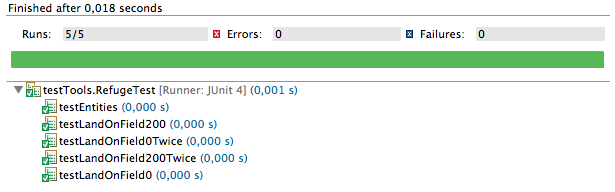
\includegraphics[width=0.8\textwidth]{RefugeTest.jpg}
\caption[<Text for the list of figures>]{Resultatet af testkørsel Refuge}
\label{fig:testrefuge} 
\end{figure}
\subsection{Test af Laborcamp}
\texttt{LaborCampTest} er stort set magen til. Her har vi bare trukket beløbet fra på \texttt{expected}, da vores felttype nu giver en negativ konsekvens for spilleren. Samtidig har vi omdøbt pointerne til \textit{Field}, så de hedder noget med \texttt{labor}. Kørslen af testen ses i figur \vref{fig:labor}.
\begin{figure}[!ht]
\centering
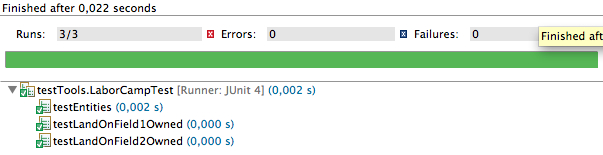
\includegraphics[width=0.8\textwidth]{LaborTest.jpg}
\caption[<Text for the list of figures>]{Resultatet af testkørsel LaborCamp}
\label{fig:labor} 
\end{figure}
\subsection{Test af Tax}
Den første testklasse til \texttt{TaxTest}, er præcis magen til \texttt{LaborCampTest}. Bortset fra vi har skiftet navnene, så de passer til denne testklasse.  Kørslen af testen ses i figur \vref{fig:testtax}.
\begin{figure}[!ht]
\centering
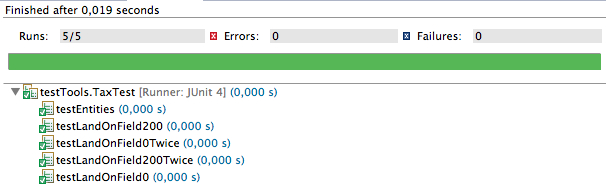
\includegraphics[width=0.8\textwidth]{TaxTest.jpg}
\caption[<Text for the list of figures>]{Resultatet af testkørsel Tax}
\label{fig:testtax} 
\end{figure}
\subsection{Test af Fleet}
Testen af \texttt{Fleet} krævede en lille smule mere arbejde. Her var vi nødt til at oprette vores \texttt{Gameboard}, for at kune sætte en ejer på vores \texttt{Fleet}. Dette gjorde vi på samme måde, som vi satte vores \texttt{player} nemlig med \texttt{this.owner = new Player(1000, "Andersine");} Vi opretter også vores \texttt{Fleet} felter \texttt{this.gameBoard.setField(new Fleet("Fleet1", 0, gameBoard), 18);}. Vi fortæller nu, hvilke felt vores \texttt{owner} har, og hvilket felt vores \texttt{player} står på, og så er det ellers stort set samme procedure som de andre tests. Kørslen af testen ses i figur \vref{fig:fleet}.
\begin{figure}[!ht]
\centering
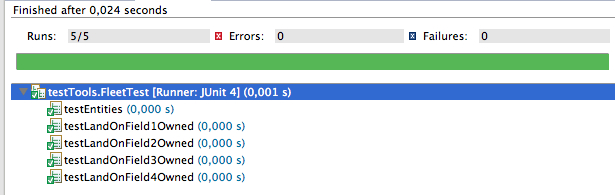
\includegraphics[width=0.8\textwidth]{FleetTest.jpg}
\caption[<Text for the list of figures>]{Resultatet af testkørsel Fleet}
\label{fig:fleet} 
\end{figure}
\subsection{Test af Territory}
Denne testklasse er bygget op på stort set samme måde som \texttt{Fleet} med en \texttt{owner} og en \texttt{player}. Det eneste specielle er at vi bliver nødt til at kalde \texttt{((Ownable)ter200).setOwner(owner);} for at kunne sætte ejeren. Kørslen af testen ses i figur \vref{fig:testter}.
\begin{figure}[!ht]
\centering
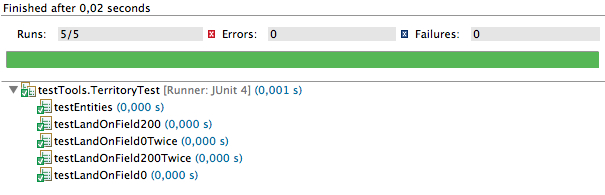
\includegraphics[width=0.8\textwidth]{TerTest.jpg}
\caption[<Text for the list of figures>]{Resultatet af testkørsel Territory}
\label{fig:testter} 
\end{figure}
\subsection{Test og fejlfinding generelt}
Vi har genbrugt vores "snydeterning" fra sidste projekt, som vi har brugt til lettere at lande på bestemte felter, når vi skulle teste en bestemt felttype.
Ellers har vi benyttet os de \textbf{White Box} tests, der var lavet en \textbf{Junit} skabelon til.

Ud over det har vi lavet en enkelt \textbf{User Test}, da al vores kode var færdig. Lige som sidst skabte det forvirring, at spillet skulle startes i Eclipse, og beskederne kom både i konsol og via \textbf{GUI}.
\newpage
\section{GRASP (General Responsibilty Assignment Software Patterns)}
Vi vil i dette afsnit beskrive de forskellige GRASP patterns, som vi har benyttet i vores program.
\subsection{Controller}
Vi har for overskueligeheden, og funktionaliteten i vores program, lavet en controller, \textit{Game}, der styrer alt hvad der sker. Alle kald og informationer der går på tværs af programmet går igennem vores kontroller uden at den egentlig har noget med nogen af signalerne at gøre udover at bestemme hvad der skal ske i de forskellige tilfælde. Man kan vel næsten sige at controlleren er vores lyskryds hvor en masse veje mødes og bliver omdirigeret.  
\subsection{Creater}
I vores program har vi gjort brug af Creatorer. Eksempelvis kan vi se på vores klasse diagram at der laves et object af en klassen \textit{Field} i \textit{Ownable}. På den måde kan vi have adgang til data fra Field uden at skulle tilgå klassen. Det er også rigtig godt for vores ønske om høj binding og lav kobling. 
\subsection{Expert}
I vores kode har der blandt andet været brug for en expert til at holde styr på vores felter på spillepladen. Derfor har vi lagret alle informationer, såsom hvad en grund koster at købe eller hvad den koster at lande på når en anden ejer den, i \textit{gameBoard} klassen. Det gør samtidigt at vi hurtigt kan komme til informationerne fra andre klasser da vi kun skal gå et sted hen for at hente informationerne. 
Man kan bruge et eksempel fra den virkelige verden. Forestil dig at du skal slå 20 dyr op. Hvis du skal slå op i en bog for hvert dyr kan det tage sin tid, i forhold til hvis du kun skal have fat i en bog.
\subsection{High Cohesion (Høj binding)}
Høj binding er noget man altid stræber efter i et system. Det har vi også gjort som man kan se på vores \textit{Account} og \textit{Player} klasser. De kender til hindanden uden at de kan gøre andet end at give kommandoer. Det vil sige at Player for eksempel kan bede om data om en spiller fra \textit{Account}, og modsat kan \textit{Account} modtage data fra \textit{Player} om en spiller. 
\subsection{Indirection}
Indirection er noget der bliver brugt i vores kode. Faktisk er vores controller \textit{Game} en indirection da den lever op til det krav at den formidler information imellem to parter der ikke kender hinanden.
\subsection{Low Coupling (Lav kobling)}
Et godt eksempel på lav kobling i vores program er imellem vores \textit{Field} og \textit{GameBoard} klasser. Her er det kun \textit{GameBoard} der kender til \textit{Field}. Generelt i vores klassediagram kan man se at der ikke er nogen returnerende pile, hvilket antyder lav kobling.
\subsection{Polymorphism}
Polymorfi bruger vi til vores \textit{Field}, \textit{Ownable}, \textit{Game}, \textit{Fleet}, \textit{LabourCamp}, og \textit{Territory klasser}. Polymorfi er et andet ord for nedarving til flere klasser. Vi nedarver fra Field, for at gøre vores program det mindre, hurtigere og mere overskueligt. Havde vi ikke brugt det, var vi kommet ud i en situation hvor vi ville skulle have lavet en masse ekstra kald for at hente alle data fra andre klasser.
\subsection{Protected Variations}
Vi bruger meget \textit{Protected Variations} i vores kode da det sørger for at vi ikke ved en fejl kommer til at ændre en variabel et sted hvor det ikke er intentionen. Det kan bl. a. ses i vores kode i \textit{Ownable} klassen hvor "price" er protected netop for at undgå dette. 
\subsection{Pure Fabrication}
Vores Field klasse kunne anses for at være \textit{Pure Fabrication}. Egentlig \textit{kan man godt} gøre det uden en Field klasse, det ville bare ødelægge alle former for lav kobling man ellers arbejder hårdt for at opnå i et system.
\newpage
\section{Design Sekvens Diagram}
I modsætning til de tidligere projekter, hvor der blev udarbejdet sekvensdiagram over hele det samlede systems virkemåde, er der til dette projekt alene lavet sekvensdiagram til en enkelt metode – landOnField i Fleet – som krævet i opgavebeskrivelsen. Dette skyldes, at systemet nu er så omfattende, at det dels vil være enormt tidskrævende at udvikle et designesekvensdiagram for hele systemet, og dels vil være så stort, at det næppe vil skabe andet end forvirring, og dermed give meget lidt værdi ift. omkostningerne ved udarbejdelsen.


Diagrammet over landOnField metoden i Fleet giver til gengæld et rigtig fint indblik i systemets generelle virkemåde, og er samtidigt ikke større end at det kan overskue af de fleste.


Det er værd at bemærke, at vi vælger en notationsform, hvor der ikke indtegnes retur-pile, med mindre der returneres en værdi af betydning. Dette fordi der ikke benyttes asynkrone kald i systemet, og det derfor bør være klart hvordan sekvensen foregår, selv uden returpile – således vurderer vi, at det giver bedre mening at udelade de ”tomme” returpile, idet det giver et simplere diagram, der er nemmere at overskue, uden at det forstyrrer meningen i figuren.

Desuden har vi tilladt os at slå de 4 identiske (i hvert fald i forhold til sekvensen) Fleet felter på fields-pladserne 18-21 sammen til en enkelt ”instans” på figuren – det giver mening fordi de alene bliver tilgået i en løkke, som behandler alle fire objekter ens.


I korte træk foregår sekvensen således:
\begin{enumerate}
\item Der undersøges om feltet er ejet af en spiller. Er det ikke det, sættes isOnBuyableField-”flaget” i spillerens objekt, som bevirker at spilleren senere får mulighed for at købet feltet. Metoden returnerer herefter. Er feltet ejet af en spiller laves yderligere et tjek – nemlig om feltet er ejet af den spiller som er landet på feltet – er det det, returnerer metoden. Er det ikke det, iværksættes koden til at beregne leje og overføre lejen til feltets ejer.
\item  For at beregne lejen, skal der tælles hvor mange andre Fleet felter ejeren af dette felt har. Dette sker ved at hente de andre felter fra GameBoard, og sammenligne ejeren af disse, med ejeren af dette felt. For hvert felt der matcher, tælles én op.
\item Når antallet af felter kendes, kan lejen findes. I koden sker det med en switch-sætning, men ift. sekvensen er den egentlige implementering ligegyldig – det vigtige er blot, at der findes et beløb for leje ud fra antallet af ejede Fleet felter.
\item Når lejen er udregnet, overføres beløbet fra spilleren som landede på feltet, til spilleren som ejer feltet. Overførslen sker med transferTo-metoden i Player, som samtidigt tjekker om spilleren har nok penge til at betale. Har han det, overføres beløbet, og metoden returnerer. Har han ikke det, overføres alt hvad spilleren har, og spilleren erklæres konkurs. Her er det værd at bemærke, at det faktisk er den samme metode der bruges til at lægge penge til og trække penge fra på en konto, så i praksis udføres tjekket for, om spillerens kontobalance kommer under 0 også ved modtageren af beløbet – men det er udeladt på diagrammet, idet det under normale omstændigheder altid vil gå godt, og dermed resultere i den sekvens som er illustreret. Et alternativt udfald her vil kræve uhensigtsmæssige ændringer i koden, eller deciderede platformsfejl, og vil i praksis kun være en teoretisk mulighed.
\end{enumerate}
Dette ses i figur \vref{fig:dsd}
\begin{figure}[!ht]
\centering
\includegraphics[width=1\textwidth]{DSD.pdf}
\caption[<Text for the list of figures>]{Design Sekvens Diagram}
\label{fig:dsd}
\end{figure}
\newpage
\section{Design-klassediagram}
Her kan man se vores Design Klasse Diagram. Hvis man kigger nok på det, vil man se at der er masser af pile, men ingen af dem har nogen der går retur. Det vil sige det er lykkedes os på en nogenlundef ornuftig måde at overholde de fleste patterns i \textbf{GRASP}.
Dette ses i figur \vref{fig:design}.
\begin{figure}[!ht]
\centering
\includegraphics[width=1\textwidth]{ClassDiagram.pdf}
\caption[<Text for the list of figures>]{Design-Klassediagram}
\label{fig:design}
\end{figure}
\newpage
\section{Kildeliste}
Her vil vi oplyse om hvilke kilder, der er brugt til rapporten.
Vi vil både oplyse om hvilke bøger, hjemmesider og software vi har brugt.
\printbibliography %Print the bibliography set under \bibliography.
\section{Anvendte værktøjer}
\begin{itemize}
\item \textbf{Eclipse - kepler}. Brugt som vores værktøj til at kode java i.
\item \textbf{UMLet}. Foretrukket værktøj til \textbf{UML} diagrammer.
\item \textbf{Dropbox}. Brugt til at dele filer imellem os. 
\item \textbf{TexMaker}. Brugt for at skabe en flot rapport skrevet i \LaTeX
\end{itemize}
\newpage
\section{Bilag}
\subsection{Kode}
Her vil hele vores kode til programmet være repræsenteret som bilag.
\subsubsection{TUI - Boundary}
\lstinputlisting[language = Java, tabsize = 2,stringstyle=\color{myblue},commentstyle=\color{mygreen},showstringspaces = false, breaklines=true, numbers = left,keywordstyle = \bfseries\color{mymauve}]{TUI.java}
\subsubsection{Graphic - Boundary}
\lstinputlisting[language = Java, tabsize = 2,stringstyle=\color{myblue},commentstyle=\color{mygreen},showstringspaces = false, breaklines=true, numbers = left,keywordstyle = \bfseries\color{mymauve}]{Graphic.java}
\subsubsection{Main - Controller}
\lstinputlisting[language = Java, tabsize = 2,stringstyle=\color{myblue},commentstyle=\color{mygreen},showstringspaces = false, breaklines=true ,numbers = left,keywordstyle = \bfseries\color{mymauve}]{Main.java}
\subsubsection{Game - Controller}
\lstinputlisting[language = Java, tabsize = 2,stringstyle=\color{myblue},commentstyle=\color{mygreen},showstringspaces = false, breaklines=true, numbers = left,keywordstyle = \bfseries\color{mymauve}]{Game.java}
\subsubsection{Player - Entity}
\lstinputlisting[language = Java, tabsize = 2,stringstyle=\color{myblue},commentstyle=\color{mygreen},showstringspaces = false, breaklines=true, numbers = left,keywordstyle = \bfseries\color{mymauve}]{Player.java}
\subsubsection{Account - Entity}
\lstinputlisting[language = Java, tabsize = 2,stringstyle=\color{myblue},commentstyle=\color{mygreen},showstringspaces = false,breaklines=true, numbers = left,keywordstyle = \bfseries\color{mymauve}]{Account.java}
\subsubsection{Gameboard - Entity}
\lstinputlisting[language = Java, tabsize = 2,stringstyle=\color{myblue},commentstyle=\color{mygreen},showstringspaces = false,breaklines=true, numbers = left,keywordstyle = \bfseries\color{mymauve}]{Gameboard.java}
\subsubsection{Field - Entity}
\lstinputlisting[language = Java, tabsize = 2,stringstyle=\color{myblue},commentstyle=\color{mygreen},showstringspaces = false,breaklines=true, numbers = left,keywordstyle = \bfseries\color{mymauve}]{Field.java}
\subsubsection{Ownable - Entity}
\lstinputlisting[language = Java, tabsize = 2,stringstyle=\color{myblue},commentstyle=\color{mygreen},showstringspaces = false,breaklines=true, numbers = left,keywordstyle = \bfseries\color{mymauve}]{Ownable.java}
\subsubsection{Fleet - Entity}
\lstinputlisting[language = Java, tabsize = 2,stringstyle=\color{myblue},commentstyle=\color{mygreen},showstringspaces = false,breaklines=true, numbers = left,keywordstyle = \bfseries\color{mymauve}]{Fleet.java}
\subsubsection{LaborCamp - Entity}
\lstinputlisting[language = Java, tabsize = 2,stringstyle=\color{myblue},commentstyle=\color{mygreen},showstringspaces = false,breaklines=true, numbers = left,keywordstyle = \bfseries\color{mymauve}]{LaborCamp.java}
\subsubsection{Refuge - Entity}
\lstinputlisting[language = Java, tabsize = 2,stringstyle=\color{myblue},commentstyle=\color{mygreen},showstringspaces = false,breaklines=true, numbers = left,keywordstyle = \bfseries\color{mymauve}]{Refuge.java}
\subsubsection{Tax - Entity}
\lstinputlisting[language = Java, tabsize = 2,stringstyle=\color{myblue},commentstyle=\color{mygreen},showstringspaces = false,breaklines=true, numbers = left,keywordstyle = \bfseries\color{mymauve}]{Tax.java}
\subsubsection{Territory - Entity}
\lstinputlisting[language = Java, tabsize = 2,stringstyle=\color{myblue},commentstyle=\color{mygreen},showstringspaces = false,breaklines=true, numbers = left,keywordstyle = \bfseries\color{mymauve}]{Territory.java}
\subsubsection{DieCup - Entity}
\lstinputlisting[language = Java, tabsize = 2,stringstyle=\color{myblue},commentstyle=\color{mygreen},showstringspaces = false, breaklines=true, numbers = left,keywordstyle = \bfseries\color{mymauve}]{DieCup.java}
\subsubsection{Die - Entity}
\lstinputlisting[language = Java, tabsize = 2,stringstyle=\color{myblue},commentstyle=\color{mygreen},showstringspaces = false,breaklines=true, numbers = left,keywordstyle = \bfseries\color{mymauve}]{Die.java}
\subsubsection{DieCupTestEntity - TestTools}
\lstinputlisting[language = Java, tabsize = 2,stringstyle=\color{myblue},commentstyle=\color{mygreen},showstringspaces = false, breaklines=true, numbers = left,keywordstyle = \bfseries\color{mymauve}]{DieCupTestEntity.java}
\subsubsection{FleetTest - TestTools}
\lstinputlisting[language = Java, tabsize = 2,stringstyle=\color{myblue},commentstyle=\color{mygreen},showstringspaces = false, breaklines=true, numbers = left,keywordstyle = \bfseries\color{mymauve}]{FleetTest.java}
\subsubsection{LaborCampTest - TestTools}
\lstinputlisting[language = Java, tabsize = 2,stringstyle=\color{myblue},commentstyle=\color{mygreen},showstringspaces = false, breaklines=true, numbers = left,keywordstyle = \bfseries\color{mymauve}]{LaborCampTest.java}
\subsubsection{RefugeTest - TestTools}
\lstinputlisting[language = Java, tabsize = 2,stringstyle=\color{myblue},commentstyle=\color{mygreen},showstringspaces = false, breaklines=true, numbers = left,keywordstyle = \bfseries\color{mymauve}]{RefugeTest.java}
\subsubsection{TaxTest - TestTools}
\lstinputlisting[language = Java, tabsize = 2,stringstyle=\color{myblue},commentstyle=\color{mygreen},showstringspaces = false, breaklines=true, numbers = left,keywordstyle = \bfseries\color{mymauve}]{TaxTest.java}
\subsubsection{TerritoryTest - TestTools}
\lstinputlisting[language = Java, tabsize = 2,stringstyle=\color{myblue},commentstyle=\color{mygreen},showstringspaces = false, breaklines=true, numbers = left,keywordstyle = \bfseries\color{mymauve}]{TerritoryTest.java}
\end{document}